% ============================================
% Unity Catalog - Databricks Beamer Presentation
% Day 8: Comprehensive Guide - Fixed Alignment
% ============================================

\documentclass[aspectratio=169]{beamer}

% ============================================
% PACKAGES
% ============================================
\usepackage{tikz}
\usepackage{graphicx}
\usepackage{hyperref}
\usepackage{xcolor}
\usepackage{fancyhdr}
\usepackage{fontspec}
\usepackage{booktabs}
\usepackage{array}
\usepackage{colortbl}
\usepackage{listings}
\usepackage{ragged2e}

% ============================================
% DATABRICKS COLOR PALETTE
% ============================================
\definecolor{databricksBlue}{RGB}{41, 49, 66}
\definecolor{databricksRed}{RGB}{220, 53, 69}
\definecolor{databricksYellow}{RGB}{255, 193, 7}
\definecolor{databricksGreen}{RGB}{76, 175, 80}
\definecolor{databricksGray}{RGB}{128, 128, 128}
\definecolor{databricksLightGray}{RGB}{245, 245, 245}
\definecolor{databricksWhite}{RGB}{255, 255, 255}
\definecolor{bronzeColor}{RGB}{205, 127, 50}
\definecolor{silverColor}{RGB}{192, 192, 192}
\definecolor{goldColor}{RGB}{255, 215, 0}

% ============================================
% BEAMER THEME CONFIGURATION
% ============================================
\usetheme{default}
\usecolortheme{default}

% Set colors
\setbeamercolor{structure}{fg=databricksBlue}
\setbeamercolor{background canvas}{bg=databricksWhite}
\setbeamercolor{normal text}{fg=databricksBlue}
\setbeamercolor{frametitle}{fg=databricksWhite,bg=databricksBlue}
\setbeamercolor{title}{fg=databricksWhite}
\setbeamercolor{subtitle}{fg=databricksLightGray}
\setbeamercolor{author}{fg=databricksWhite}
\setbeamercolor{date}{fg=databricksLightGray}
\setbeamercolor{item}{fg=databricksBlue}
\setbeamercolor{subitem}{fg=databricksRed}
\setbeamercolor{block title}{fg=databricksWhite,bg=databricksBlue}
\setbeamercolor{block body}{fg=databricksBlue,bg=databricksLightGray}
\setbeamercolor{block title example}{fg=databricksWhite,bg=databricksGreen}
\setbeamercolor{block body example}{fg=databricksBlue,bg=databricksLightGray}
\setbeamercolor{block title alerted}{fg=databricksWhite,bg=databricksRed}
\setbeamercolor{block body alerted}{fg=databricksBlue,bg=databricksLightGray}

% Remove navigation symbols
\setbeamertemplate{navigation symbols}{}

% Set fonts
\setbeamerfont{title}{size=\Huge,series=\bfseries}
\setbeamerfont{subtitle}{size=\large}
\setbeamerfont{frametitle}{size=\Large,series=\bfseries}
\setbeamerfont{framesubtitle}{size=\normalsize}

% ============================================
% CUSTOM TEMPLATES
% ============================================

% Title page
\setbeamertemplate{title page}{
    \begin{tikzpicture}[remember picture,overlay]
        \fill[databricksBlue] (current page.north west) rectangle (current page.south east);
        \node[anchor=center] at (current page.center) {
            \begin{minipage}{0.9\textwidth}
                \centering
                {\usebeamerfont{title}\usebeamercolor[fg]{title}\inserttitle\par}
                \vspace{0.5cm}
                {\usebeamerfont{subtitle}\usebeamercolor[fg]{subtitle}\insertsubtitle\par}
                \vspace{1cm}
                {\usebeamerfont{author}\usebeamercolor[fg]{author}\insertauthor\par}
                \vspace{0.3cm}
                {\usebeamerfont{date}\usebeamercolor[fg]{date}\insertdate\par}
            \end{minipage}
        };
    \end{tikzpicture}
}

% Frame title
\setbeamertemplate{frametitle}{
    \begin{beamercolorbox}[wd=\paperwidth,ht=1.2cm,dp=0.3cm,leftskip=0.5cm]{frametitle}
        \usebeamerfont{frametitle}\insertframetitle
    \end{beamercolorbox}
}

% Footer
\setbeamertemplate{footline}{
    \begin{tikzpicture}[remember picture,overlay]
        \fill[databricksBlue] (current page.south west) rectangle ([yshift=0.6cm]current page.south east);
        \node[anchor=west,xshift=0.5cm,yshift=0.3cm,font=\tiny\color{white}] at (current page.south west) {
            \href{https://easy-ai-labs.lovable.app/}{\textcolor{white}{Easy AI Labs}}
        };
        \node[anchor=center,yshift=0.3cm,font=\tiny\color{white}] at (current page.south) {
            \href{https://www.linkedin.com/in/yashkavaiya}{\textcolor{white}{Yash Kavaiya}}
        };
        \node[anchor=east,xshift=-1.5cm,yshift=0.3cm,font=\tiny\color{white}] at (current page.south east) {
            \href{https://www.linkedin.com/company/genai-guru}{\textcolor{white}{Gen AI Guru}}
        };
        \node[anchor=east,xshift=-0.3cm,yshift=0.3cm,font=\tiny\color{white}] at (current page.south east) {
            \insertframenumber/\inserttotalframenumber
        };
    \end{tikzpicture}
}

% Custom itemize
\setbeamertemplate{itemize item}{\textcolor{databricksBlue}{$\bullet$}}
\setbeamertemplate{itemize subitem}{\textcolor{databricksRed}{$\triangleright$}}
\setbeamertemplate{itemize subsubitem}{\textcolor{databricksGreen}{$\circ$}}

% Code listings style
\lstset{
    basicstyle=\ttfamily\tiny,
    keywordstyle=\color{databricksBlue}\bfseries,
    commentstyle=\color{databricksGray},
    stringstyle=\color{databricksGreen},
    breaklines=true,
    frame=single,
    backgroundcolor=\color{databricksLightGray},
    rulecolor=\color{databricksBlue},
    showstringspaces=false
}

% ============================================
% DOCUMENT METADATA
% ============================================
\title{Unity Catalog}
\subtitle{Comprehensive Guide to Unified Data Governance}
\author{Databricks 14-Days AI Challenge}
\date{Day 8}

% ============================================
% DOCUMENT CONTENT
% ============================================
\begin{document}

% Title Slide
\frame{\titlepage}

% ============================================
% Table of Contents
% ============================================
\begin{frame}{Agenda}
    \begin{columns}[T]
        \begin{column}{0.48\textwidth}
            \begin{itemize}
                \item \textcolor{databricksBlue}{\textbf{Introduction}} to Unity Catalog
                \item \textcolor{databricksBlue}{\textbf{Three-Level Namespace}} Hierarchy
                \item \textcolor{databricksBlue}{\textbf{Catalog → Schema → Table}}
                \item \textcolor{databricksBlue}{\textbf{Managed vs External}} Tables
            \end{itemize}
        \end{column}
        \begin{column}{0.48\textwidth}
            \begin{itemize}
                \item \textcolor{databricksBlue}{\textbf{Access Control}} with GRANT/REVOKE
                \item \textcolor{databricksBlue}{\textbf{Data Lineage}}
                \item \textcolor{databricksBlue}{\textbf{Practical Implementation}}
                \item \textcolor{databricksBlue}{\textbf{Best Practices}}
            \end{itemize}
        \end{column}
    \end{columns}
\end{frame}

% ============================================
% SECTION: Introduction
% ============================================
\begin{frame}{What is Unity Catalog?}
    \begin{block}{Definition}
        Unity Catalog is Databricks' \textcolor{databricksRed}{\textbf{unified governance solution}} for all data and AI assets.
    \end{block}
    \vspace{0.3cm}
    \textbf{Think of it as:}
    \begin{itemize}
        \item The \textcolor{databricksBlue}{\textbf{central librarian}} for your entire data ecosystem
        \item It knows \textcolor{databricksGreen}{\textbf{where everything is stored}}
        \item It controls \textcolor{databricksYellow}{\textbf{who can access what}}
        \item It tracks \textcolor{databricksRed}{\textbf{how data flows}} through your organization
    \end{itemize}
\end{frame}

% ============================================
\begin{frame}{Why Unity Catalog Matters}
    \small
    \begin{center}
        \begin{tabular}{>{\raggedright\arraybackslash}p{2.8cm}>{\raggedright\arraybackslash}p{4.2cm}>{\raggedright\arraybackslash}p{4.2cm}}
            \toprule
            \rowcolor{databricksBlue}\textcolor{white}{\textbf{Challenge}} & \textcolor{white}{\textbf{Without Unity Catalog}} & \textcolor{white}{\textbf{With Unity Catalog}} \\
            \midrule
            \textbf{Data Discovery} & Scattered metadata & Single searchable catalog \\
            \rowcolor{databricksLightGray}\textbf{Access Control} & Inconsistent, workspace-specific & Centralized, consistent \\
            \textbf{Audit Trail} & Limited visibility & Complete lineage \& logs \\
            \rowcolor{databricksLightGray}\textbf{Data Sharing} & Complex, insecure & Secure, governed \\
            \textbf{Compliance} & Manual tracking & Automated reporting \\
            \bottomrule
        \end{tabular}
    \end{center}
\end{frame}

% ============================================
\begin{frame}{Core Capabilities}
    \begin{columns}[T]
        \begin{column}{0.48\textwidth}
            \begin{block}{1. Centralized Governance}
                Single place to manage \textcolor{databricksBlue}{\textbf{all data assets}}
            \end{block}
            \vspace{0.3cm}
            \begin{block}{2. Fine-grained Access Control}
                Control who can do what, \textcolor{databricksRed}{\textbf{at any level}}
            \end{block}
        \end{column}
        \begin{column}{0.48\textwidth}
            \begin{block}{3. Data Lineage}
                Track where data \textcolor{databricksGreen}{\textbf{comes from}} and \textcolor{databricksGreen}{\textbf{goes}}
            \end{block}
            \vspace{0.3cm}
            \begin{block}{4. Data Sharing}
                \textcolor{databricksYellow}{\textbf{Securely share}} data across organizations
            \end{block}
        \end{column}
    \end{columns}
\end{frame}

% ============================================
% SECTION: Three-Level Namespace
% ============================================
\begin{frame}{Three-Level Namespace Hierarchy}
    \begin{center}
        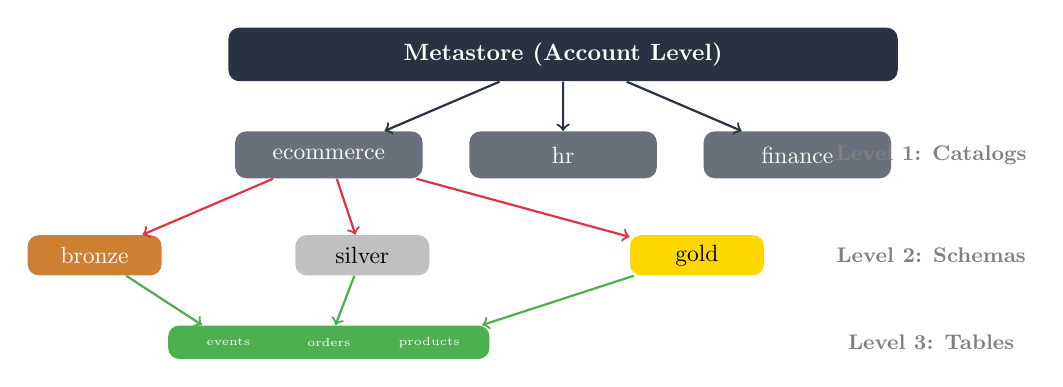
\begin{tikzpicture}[scale=0.85, transform shape]
            % Metastore
            \node[fill=databricksBlue,text=white,rounded corners,minimum width=10cm,minimum height=0.8cm] (meta) at (0,4) {\textbf{Metastore (Account Level)}};
            
            % Catalogs
            \node[fill=databricksBlue!70,text=white,rounded corners,minimum width=2.8cm,minimum height=0.7cm] (cat1) at (-3.5,2.5) {ecommerce};
            \node[fill=databricksBlue!70,text=white,rounded corners,minimum width=2.8cm,minimum height=0.7cm] (cat2) at (0,2.5) {hr};
            \node[fill=databricksBlue!70,text=white,rounded corners,minimum width=2.8cm,minimum height=0.7cm] (cat3) at (3.5,2.5) {finance};
            
            % Schemas
            \node[fill=bronzeColor,text=white,rounded corners,minimum width=2cm,minimum height=0.6cm] (sch1) at (-7,1) {bronze};
            \node[fill=silverColor,text=black,rounded corners,minimum width=2cm,minimum height=0.6cm] (sch2) at (-3,1) {silver};
            \node[fill=goldColor,text=black,rounded corners,minimum width=2cm,minimum height=0.6cm] (sch3) at (2,1) {gold};
            
            % Tables
            \node[fill=databricksGreen,text=white,rounded corners,minimum width=1.8cm,minimum height=0.5cm,font=\tiny] (tbl1) at (-5,-0.3) {events};
            \node[fill=databricksGreen,text=white,rounded corners,minimum width=1.8cm,minimum height=0.5cm,font=\tiny] (tbl2) at (-3.5,-0.3) {orders};
            \node[fill=databricksGreen,text=white,rounded corners,minimum width=1.8cm,minimum height=0.5cm,font=\tiny] (tbl3) at (-2,-0.3) {products};
            
            % Connections
            \draw[->,thick,databricksBlue] (meta) -- (cat1);
            \draw[->,thick,databricksBlue] (meta) -- (cat2);
            \draw[->,thick,databricksBlue] (meta) -- (cat3);
            \draw[->,thick,databricksRed] (cat1) -- (sch1);
            \draw[->,thick,databricksRed] (cat1) -- (sch2);
            \draw[->,thick,databricksRed] (cat1) -- (sch3);
            \draw[->,thick,databricksGreen] (sch1) -- (tbl1);
            \draw[->,thick,databricksGreen] (sch2) -- (tbl2);
            \draw[->,thick,databricksGreen] (sch3) -- (tbl3);
            
            % Labels
            \node[font=\small,databricksGray] at (5.5,2.5) {\textbf{Level 1: Catalogs}};
            \node[font=\small,databricksGray] at (5.5,1) {\textbf{Level 2: Schemas}};
            \node[font=\small,databricksGray] at (5.5,-0.3) {\textbf{Level 3: Tables}};
        \end{tikzpicture}
    \end{center}
\end{frame}

% ============================================
\begin{frame}{The Complete Address Format}
    \begin{block}{Fully Qualified Name Pattern}
        \centering
        \texttt{\Large \textcolor{databricksBlue}{catalog}.\textcolor{databricksRed}{schema}.\textcolor{databricksGreen}{table}}
    \end{block}
    \vspace{0.3cm}
    \begin{center}
        \textbf{Example:} \texttt{ecommerce.gold.products}
    \end{center}
    \vspace{0.3cm}
    \small
    \begin{center}
        \begin{tabular}{>{\centering\arraybackslash}p{2.2cm}>{\centering\arraybackslash}p{2.2cm}>{\centering\arraybackslash}p{2.5cm}>{\centering\arraybackslash}p{3.5cm}}
            \toprule
            \rowcolor{databricksBlue}\textcolor{white}{\textbf{Level}} & \textcolor{white}{\textbf{Analogy}} & \textcolor{white}{\textbf{Example}} & \textcolor{white}{\textbf{Purpose}} \\
            \midrule
            Metastore & Country & (Implicit) & Top-level container \\
            \rowcolor{databricksLightGray}Catalog & City & \texttt{ecommerce} & Groups by domain \\
            Schema & Street & \texttt{gold} & Groups by data layer \\
            \rowcolor{databricksLightGray}Table & House & \texttt{products} & Actual data \\
            \bottomrule
        \end{tabular}
    \end{center}
\end{frame}

% ============================================
% SECTION: Catalog, Schema, Table
% ============================================
\begin{frame}{Level 1: Catalog}
    \begin{columns}[T]
        \begin{column}{0.52\textwidth}
            \textbf{Key Characteristics:}
            \begin{itemize}
                \item First component of three-part naming
                \item Contains \textcolor{databricksBlue}{\textbf{multiple schemas}}
                \item \textcolor{databricksRed}{\textbf{Isolation boundary}} for permissions
                \item Represents a \textcolor{databricksGreen}{\textbf{business domain}}
            \end{itemize}
        \end{column}
        \begin{column}{0.44\textwidth}
            \begin{exampleblock}{Creating a Catalog}
                \texttt{\footnotesize CREATE CATALOG ecommerce}\\
                \texttt{\footnotesize COMMENT 'E-commerce data';}\\
                \vspace{0.2cm}
                \texttt{\footnotesize USE CATALOG ecommerce;}
            \end{exampleblock}
        \end{column}
    \end{columns}
    \vspace{0.4cm}
    \textbf{Catalog Strategies:}
    \small
    \begin{center}
        \begin{tabular}{>{\centering\arraybackslash}p{3.5cm}>{\centering\arraybackslash}p{3.5cm}>{\centering\arraybackslash}p{3.5cm}}
            \toprule
            \textcolor{databricksBlue}{\textbf{By Domain}} & \textcolor{databricksRed}{\textbf{By Environment}} & \textcolor{databricksGreen}{\textbf{By Region}} \\
            \midrule
            ecommerce, marketing & dev, staging, prod & us\_west, eu\_central \\
            \bottomrule
        \end{tabular}
    \end{center}
\end{frame}

% ============================================
\begin{frame}{Level 2: Schema - Medallion Architecture}
    \begin{center}
        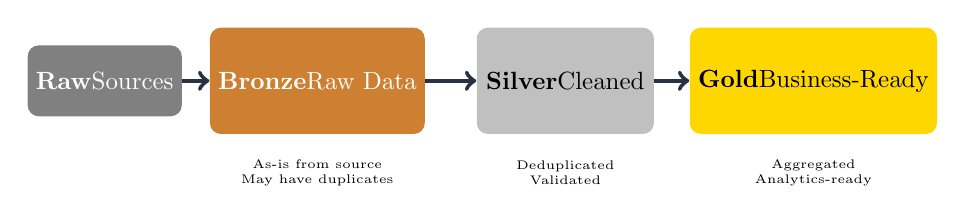
\begin{tikzpicture}[scale=0.9, transform shape]
            % Data flow
            \node[fill=databricksGray,text=white,rounded corners,minimum width=2cm,minimum height=1cm] (raw) at (-5,0) {\textbf{Raw}\\Sources};
            
            \node[fill=bronzeColor,text=white,rounded corners,minimum width=2.5cm,minimum height=1.5cm] (bronze) at (-2,0) {\textbf{Bronze}\\Raw Data};
            
            \node[fill=silverColor,text=black,rounded corners,minimum width=2.5cm,minimum height=1.5cm] (silver) at (1.5,0) {\textbf{Silver}\\Cleaned};
            
            \node[fill=goldColor,text=black,rounded corners,minimum width=2.5cm,minimum height=1.5cm] (gold) at (5,0) {\textbf{Gold}\\Business-Ready};
            
            \draw[->,ultra thick,databricksBlue] (raw) -- (bronze);
            \draw[->,ultra thick,databricksBlue] (bronze) -- (silver);
            \draw[->,ultra thick,databricksBlue] (silver) -- (gold);
            
            % Labels below
            \node[font=\tiny,align=center] at (-2,-1.3) {As-is from source\\May have duplicates};
            \node[font=\tiny,align=center] at (1.5,-1.3) {Deduplicated\\Validated};
            \node[font=\tiny,align=center] at (5,-1.3) {Aggregated\\Analytics-ready};
        \end{tikzpicture}
    \end{center}
    \vspace{0.4cm}
    \begin{exampleblock}{Creating Schemas}
        \texttt{\footnotesize CREATE SCHEMA bronze COMMENT 'Raw ingested data';}\\
        \texttt{\footnotesize CREATE SCHEMA silver COMMENT 'Cleaned data';}\\
        \texttt{\footnotesize CREATE SCHEMA gold COMMENT 'Business-ready aggregations';}
    \end{exampleblock}
\end{frame}

% ============================================
\begin{frame}{Level 3: Tables and Views}
    \small
    \begin{center}
        \begin{tabular}{>{\raggedright\arraybackslash}p{3.2cm}>{\raggedright\arraybackslash}p{5cm}>{\centering\arraybackslash}p{2.2cm}}
            \toprule
            \rowcolor{databricksBlue}\textcolor{white}{\textbf{Object Type}} & \textcolor{white}{\textbf{Description}} & \textcolor{white}{\textbf{Stores Data?}} \\
            \midrule
            Managed Table & UC manages metadata \& data files & \textcolor{databricksGreen}{\textbf{Yes}} \\
            \rowcolor{databricksLightGray}External Table & UC manages only metadata & \textcolor{databricksYellow}{\textbf{External}} \\
            View & Saved SQL query & \textcolor{databricksRed}{\textbf{No}} \\
            \rowcolor{databricksLightGray}Materialized View & Precomputed view stored as table & \textcolor{databricksGreen}{\textbf{Yes}} \\
            Function & User-defined functions (UDFs) & \textcolor{databricksRed}{\textbf{No}} \\
            \bottomrule
        \end{tabular}
    \end{center}
    \begin{exampleblock}{Creating a Managed Table}
        \texttt{\footnotesize CREATE TABLE bronze.events (}\\
        \texttt{\footnotesize \ \ event\_id STRING, user\_id STRING, event\_timestamp TIMESTAMP}\\
        \texttt{\footnotesize ) USING DELTA;}
    \end{exampleblock}
\end{frame}

% ============================================
% SECTION: Managed vs External Tables
% ============================================
\begin{frame}{Managed vs External Tables}
    \begin{center}
        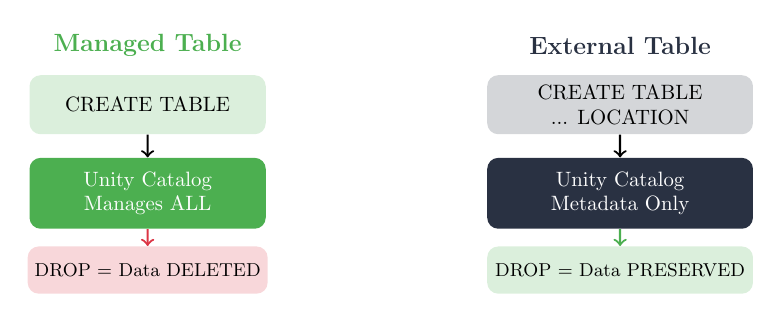
\begin{tikzpicture}[scale=0.75, transform shape]
            % Managed Table
            \node[font=\large\bfseries,databricksGreen] at (-4,3) {Managed Table};
            \node[fill=databricksGreen!20,rounded corners,minimum width=4cm,minimum height=1cm] (m1) at (-4,2) {CREATE TABLE};
            \node[fill=databricksGreen,text=white,rounded corners,minimum width=4cm,minimum height=1.2cm,align=center] (m2) at (-4,0.5) {Unity Catalog\\Manages ALL};
            \node[fill=databricksRed!20,rounded corners,minimum width=4cm,minimum height=0.8cm,font=\small] (m3) at (-4,-0.8) {DROP = Data DELETED};
            
            \draw[->,thick] (m1) -- (m2);
            \draw[->,thick,databricksRed] (m2) -- (m3);
            
            % External Table
            \node[font=\large\bfseries,databricksBlue] at (4,3) {External Table};
            \node[fill=databricksBlue!20,rounded corners,minimum width=4.5cm,minimum height=1cm,align=center] (e1) at (4,2) {CREATE TABLE\\... LOCATION};
            \node[fill=databricksBlue,text=white,rounded corners,minimum width=4.5cm,minimum height=1.2cm,align=center] (e2) at (4,0.5) {Unity Catalog\\Metadata Only};
            \node[fill=databricksGreen!20,rounded corners,minimum width=4.5cm,minimum height=0.8cm,font=\small] (e3) at (4,-0.8) {DROP = Data PRESERVED};
            
            \draw[->,thick] (e1) -- (e2);
            \draw[->,thick,databricksGreen] (e2) -- (e3);
        \end{tikzpicture}
    \end{center}
\end{frame}

% ============================================
\begin{frame}{When to Use Each Type}
    \begin{columns}[T]
        \begin{column}{0.48\textwidth}
            \begin{block}{\textcolor{databricksGreen}{Choose Managed Tables}}
                \begin{itemize}
                    \item Starting \textbf{fresh} with new data
                    \item Want \textbf{automatic} storage handling
                    \item Working on \textbf{isolated} projects
                    \item Want \textbf{automatic cleanup} on delete
                    \item \textbf{Simplicity} is priority
                \end{itemize}
            \end{block}
        \end{column}
        \begin{column}{0.48\textwidth}
            \begin{block}{\textcolor{databricksBlue}{Choose External Tables}}
                \begin{itemize}
                    \item Have \textbf{existing} data in cloud storage
                    \item \textbf{Multiple systems} access same files
                    \item Want to \textbf{preserve} data after drop
                    \item \textbf{Migrating} from existing data lake
                    \item Need \textbf{control} over storage location
                \end{itemize}
            \end{block}
        \end{column}
    \end{columns}
\end{frame}

% ============================================
% SECTION: Access Control
% ============================================
\begin{frame}{Access Control - The Security Model}
    \begin{center}
        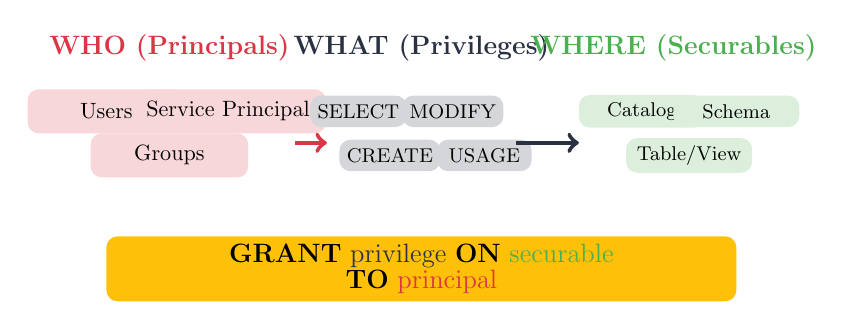
\begin{tikzpicture}[scale=0.8, transform shape]
            % WHO
            \node[font=\large\bfseries,databricksRed] at (-4,3.5) {WHO (Principals)};
            \node[fill=databricksRed!20,rounded corners,minimum width=2.5cm,minimum height=0.7cm] at (-5,2.5) {Users};
            \node[fill=databricksRed!20,rounded corners,minimum width=2.5cm,minimum height=0.7cm] at (-4,1.8) {Groups};
            \node[fill=databricksRed!20,rounded corners,minimum width=2.5cm,minimum height=0.7cm] at (-3,2.5) {Service Principals};
            
            % WHAT
            \node[font=\large\bfseries,databricksBlue] at (0,3.5) {WHAT (Privileges)};
            \node[fill=databricksBlue!20,rounded corners,minimum width=1.5cm,minimum height=0.5cm,font=\small] at (-1,2.5) {SELECT};
            \node[fill=databricksBlue!20,rounded corners,minimum width=1.5cm,minimum height=0.5cm,font=\small] at (0.5,2.5) {MODIFY};
            \node[fill=databricksBlue!20,rounded corners,minimum width=1.5cm,minimum height=0.5cm,font=\small] at (-0.5,1.8) {CREATE};
            \node[fill=databricksBlue!20,rounded corners,minimum width=1.5cm,minimum height=0.5cm,font=\small] at (1,1.8) {USAGE};
            
            % WHERE
            \node[font=\large\bfseries,databricksGreen] at (4,3.5) {WHERE (Securables)};
            \node[fill=databricksGreen!20,rounded corners,minimum width=2cm,minimum height=0.5cm,font=\small] at (3.5,2.5) {Catalog};
            \node[fill=databricksGreen!20,rounded corners,minimum width=2cm,minimum height=0.5cm,font=\small] at (5,2.5) {Schema};
            \node[fill=databricksGreen!20,rounded corners,minimum width=2cm,minimum height=0.5cm,font=\small] at (4.25,1.8) {Table/View};
            
            % Arrows
            \draw[->,ultra thick,databricksRed] (-2,2) -- (-1.5,2);
            \draw[->,ultra thick,databricksBlue] (1.5,2) -- (2.5,2);
            
            % Formula
            \node[fill=databricksYellow,rounded corners,minimum width=10cm,minimum height=1cm,font=\large,align=center] at (0,0) {\textbf{GRANT} \textcolor{databricksBlue}{privilege} \textbf{ON} \textcolor{databricksGreen}{securable}\\[-2pt]\textbf{TO} \textcolor{databricksRed}{principal}};
        \end{tikzpicture}
    \end{center}
\end{frame}

% ============================================
\begin{frame}{Key Privileges}
    \small
    \begin{center}
        \begin{tabular}{>{\raggedright\arraybackslash}p{2.5cm}>{\raggedright\arraybackslash}p{5.8cm}>{\raggedright\arraybackslash}p{2.5cm}}
            \toprule
            \rowcolor{databricksBlue}\textcolor{white}{\textbf{Privilege}} & \textcolor{white}{\textbf{Description}} & \textcolor{white}{\textbf{Applies To}} \\
            \midrule
            \texttt{SELECT} & Read data from tables/views & Tables, Views \\
            \rowcolor{databricksLightGray}\texttt{MODIFY} & Add, update, delete data & Tables \\
            \texttt{CREATE} & Create objects within container & Catalogs, Schemas \\
            \rowcolor{databricksLightGray}\texttt{USAGE} & Access the container (required) & Catalogs, Schemas \\
            \texttt{ALL PRIVILEGES} & All available privileges & All securables \\
            \rowcolor{databricksLightGray}\texttt{EXECUTE} & Run functions & Functions \\
            \bottomrule
        \end{tabular}
    \end{center}
    \begin{alertblock}{Important}
        \texttt{USAGE} on parent containers is \textcolor{databricksRed}{\textbf{required}} before granting table-level privileges!
    \end{alertblock}
\end{frame}

% ============================================
\begin{frame}{Privilege Inheritance}
    \begin{center}
        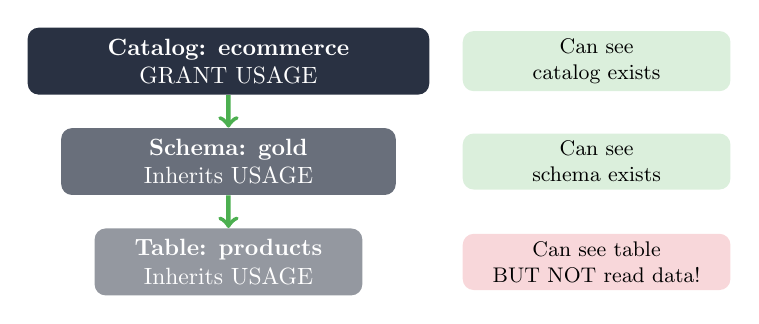
\begin{tikzpicture}[scale=0.85, transform shape]
            % Hierarchy
            \node[fill=databricksBlue,text=white,rounded corners,minimum width=6cm,minimum height=1cm,align=center] (cat) at (0,3) {\textbf{Catalog: ecommerce}\\GRANT USAGE};
            
            \node[fill=databricksBlue!70,text=white,rounded corners,minimum width=5cm,minimum height=1cm,align=center] (sch) at (0,1.5) {\textbf{Schema: gold}\\Inherits USAGE};
            
            \node[fill=databricksBlue!50,text=white,rounded corners,minimum width=4cm,minimum height=1cm,align=center] (tbl) at (0,0) {\textbf{Table: products}\\Inherits USAGE};
            
            \draw[->,ultra thick,databricksGreen] (cat) -- (sch);
            \draw[->,ultra thick,databricksGreen] (sch) -- (tbl);
            
            % Access notes
            \node[fill=databricksGreen!20,rounded corners,minimum width=4cm,font=\small,align=center] at (5.5,3) {Can see\\catalog exists};
            \node[fill=databricksGreen!20,rounded corners,minimum width=4cm,font=\small,align=center] at (5.5,1.5) {Can see\\schema exists};
            \node[fill=databricksRed!20,rounded corners,minimum width=4cm,font=\small,align=center] at (5.5,0) {Can see table\\BUT NOT read data!};
        \end{tikzpicture}
    \end{center}
    \vspace{0.3cm}
    \textbf{To read data:} \texttt{USAGE} on Catalog + \texttt{USAGE} on Schema + \texttt{SELECT} on Table
\end{frame}

% ============================================
\begin{frame}{GRANT/REVOKE Examples}
    \begin{exampleblock}{GRANT Examples}
        \texttt{\footnotesize -- Grant SELECT on specific table}\\
        \texttt{\footnotesize GRANT SELECT ON TABLE gold.products TO `analysts@company.com`;}\\[0.2cm]
        \texttt{\footnotesize -- Grant all privileges on schema}\\
        \texttt{\footnotesize GRANT ALL PRIVILEGES ON SCHEMA silver TO `engineers@company.com`;}\\[0.2cm]
        \texttt{\footnotesize -- Grant USAGE to access catalog}\\
        \texttt{\footnotesize GRANT USAGE ON CATALOG ecommerce TO `data\_team`;}
    \end{exampleblock}
    \vspace{0.3cm}
    \begin{alertblock}{REVOKE Example}
        \texttt{\footnotesize REVOKE SELECT ON TABLE gold.products FROM `intern@company.com`;}
    \end{alertblock}
\end{frame}

% ============================================
\begin{frame}{Permission Patterns}
    \begin{columns}[T]
        \begin{column}{0.48\textwidth}
            \begin{block}{Data Analysts (Read-Only Gold)}
                \texttt{\tiny GRANT USAGE ON CATALOG ecommerce}\\
                \texttt{\tiny \ \ TO `analysts@company.com`;}\\
                \texttt{\tiny GRANT USAGE ON SCHEMA gold}\\
                \texttt{\tiny \ \ TO `analysts@company.com`;}\\
                \texttt{\tiny GRANT SELECT ON ALL TABLES IN}\\
                \texttt{\tiny \ \ SCHEMA gold TO `analysts@company.com`;}
            \end{block}
        \end{column}
        \begin{column}{0.48\textwidth}
            \begin{block}{Data Engineers (Full Access)}
                \texttt{\tiny GRANT ALL PRIVILEGES ON CATALOG}\\
                \texttt{\tiny \ \ ecommerce TO `engineers@company.com`;}
            \end{block}
            \vspace{0.3cm}
            \begin{block}{Views for Controlled Access}
                Create views to expose only \textcolor{databricksGreen}{\textbf{specific columns/rows}}
            \end{block}
        \end{column}
    \end{columns}
\end{frame}

% ============================================
% SECTION: Data Lineage
% ============================================
\begin{frame}{Data Lineage}
    \begin{block}{Definition}
        Data lineage tracks the \textcolor{databricksBlue}{\textbf{complete journey of data}}—where it comes from, how it transforms, and where it ends up.
    \end{block}
    \vspace{0.3cm}
    \begin{center}
        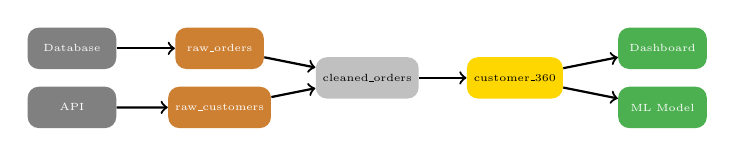
\begin{tikzpicture}[scale=0.75, transform shape]
            % Source
            \node[fill=databricksGray,text=white,rounded corners,minimum width=1.5cm,minimum height=0.7cm,font=\tiny] (s1) at (-5,0) {Database};
            \node[fill=databricksGray,text=white,rounded corners,minimum width=1.5cm,minimum height=0.7cm,font=\tiny] (s2) at (-5,-1) {API};
            
            % Bronze
            \node[fill=bronzeColor,text=white,rounded corners,minimum width=1.5cm,minimum height=0.7cm,font=\tiny] (b1) at (-2.5,0) {raw\_orders};
            \node[fill=bronzeColor,text=white,rounded corners,minimum width=1.5cm,minimum height=0.7cm,font=\tiny] (b2) at (-2.5,-1) {raw\_customers};
            
            % Silver
            \node[fill=silverColor,text=black,rounded corners,minimum width=1.5cm,minimum height=0.7cm,font=\tiny] (si1) at (0,-0.5) {cleaned\_orders};
            
            % Gold
            \node[fill=goldColor,text=black,rounded corners,minimum width=1.5cm,minimum height=0.7cm,font=\tiny] (g1) at (2.5,-0.5) {customer\_360};
            
            % Consumption
            \node[fill=databricksGreen,text=white,rounded corners,minimum width=1.5cm,minimum height=0.7cm,font=\tiny] (d1) at (5,0) {Dashboard};
            \node[fill=databricksGreen,text=white,rounded corners,minimum width=1.5cm,minimum height=0.7cm,font=\tiny] (d2) at (5,-1) {ML Model};
            
            \draw[->,thick] (s1) -- (b1);
            \draw[->,thick] (s2) -- (b2);
            \draw[->,thick] (b1) -- (si1);
            \draw[->,thick] (b2) -- (si1);
            \draw[->,thick] (si1) -- (g1);
            \draw[->,thick] (g1) -- (d1);
            \draw[->,thick] (g1) -- (d2);
        \end{tikzpicture}
    \end{center}
    \vspace{0.2cm}
    \textbf{Unity Catalog automatically captures:} Table lineage, Column lineage, Query lineage, User lineage
\end{frame}

% ============================================
\begin{frame}{Lineage Types \& Benefits}
    \begin{columns}[T]
        \begin{column}{0.48\textwidth}
            \textbf{Types of Lineage:}
            \begin{itemize}
                \item \textcolor{databricksBlue}{\textbf{Table Lineage}} - Source to target tables
                \item \textcolor{databricksRed}{\textbf{Column Lineage}} - Source to target columns
                \item \textcolor{databricksGreen}{\textbf{Query Lineage}} - Which queries access tables
                \item \textcolor{databricksYellow}{\textbf{User Lineage}} - Who interacts with data
            \end{itemize}
        \end{column}
        \begin{column}{0.48\textwidth}
            \textbf{Benefits:}
            \begin{itemize}
                \item \textcolor{databricksBlue}{\textbf{Impact Analysis}} - See downstream dependencies
                \item \textcolor{databricksRed}{\textbf{Root Cause}} - Trace data errors
                \item \textcolor{databricksGreen}{\textbf{Compliance}} - Show data provenance
                \item \textcolor{databricksYellow}{\textbf{Documentation}} - Auto-generated flows
            \end{itemize}
        \end{column}
    \end{columns}
    \vspace{0.4cm}
    \begin{block}{Viewing Lineage}
        Navigate to \textbf{Catalog} → Find your table → Click \textbf{Lineage} tab
    \end{block}
\end{frame}

% ============================================
% SECTION: Best Practices
% ============================================
\begin{frame}{Naming Conventions}
    \small
    \begin{center}
        \begin{tabular}{>{\raggedright\arraybackslash}p{2.5cm}>{\raggedright\arraybackslash}p{4cm}>{\raggedright\arraybackslash}p{4cm}}
            \toprule
            \rowcolor{databricksBlue}\textcolor{white}{\textbf{Level}} & \textcolor{white}{\textbf{Convention}} & \textcolor{white}{\textbf{Example}} \\
            \midrule
            Catalog & lowercase, business domain & \texttt{ecommerce}, \texttt{hr} \\
            \rowcolor{databricksLightGray}Schema & lowercase, data layer & \texttt{bronze}, \texttt{silver}, \texttt{gold} \\
            Table & lowercase\_snake\_case & \texttt{customer\_orders} \\
            \rowcolor{databricksLightGray}View & prefix with purpose & \texttt{rpt\_sales\_summary} \\
            \bottomrule
        \end{tabular}
    \end{center}
    \vspace{0.4cm}
    \begin{block}{Permission Best Practices}
        \begin{itemize}
            \item Use \textcolor{databricksBlue}{\textbf{Groups}}, not individual users
            \item Apply \textcolor{databricksRed}{\textbf{Principle of Least Privilege}}
            \item Use \textcolor{databricksGreen}{\textbf{Views}} for row/column filtering
            \item Conduct \textcolor{databricksYellow}{\textbf{Regular Access Reviews}}
        \end{itemize}
    \end{block}
\end{frame}

% ============================================
\begin{frame}{Anti-Patterns to Avoid}
    \small
    \begin{center}
        \begin{tabular}{>{\raggedright\arraybackslash}p{3.2cm}>{\raggedright\arraybackslash}p{3.5cm}>{\raggedright\arraybackslash}p{3.8cm}}
            \toprule
            \rowcolor{databricksRed}\textcolor{white}{\textbf{Anti-Pattern}} & \textcolor{white}{\textbf{Problem}} & \textcolor{white}{\textbf{Better Approach}} \\
            \midrule
            ALL PRIVILEGES broadly & Over-permissioning & Grant specific privileges \\
            \rowcolor{databricksLightGray}Granting to individuals & Hard to manage & Use groups \\
            Skipping USAGE grants & Tables inaccessible & Always grant USAGE first \\
            \rowcolor{databricksLightGray}One giant catalog & No isolation & Separate by domain \\
            Direct table access & No data protection & Use views \\
            \bottomrule
        \end{tabular}
    \end{center}
\end{frame}

% ============================================
\begin{frame}{Permission Quick Reference}
    \small
    \begin{center}
        \begin{tabular}{>{\raggedright\arraybackslash}p{5.5cm}>{\raggedright\arraybackslash}p{5cm}}
            \toprule
            \rowcolor{databricksBlue}\textcolor{white}{\textbf{To Do This...}} & \textcolor{white}{\textbf{Grant This...}} \\
            \midrule
            See a catalog exists & \texttt{USAGE ON CATALOG} \\
            \rowcolor{databricksLightGray}See schemas in a catalog & \texttt{USAGE ON CATALOG} \\
            See tables in a schema & \texttt{USAGE ON CATALOG + SCHEMA} \\
            \rowcolor{databricksLightGray}Read data from a table & Above + \texttt{SELECT ON TABLE} \\
            Insert/Update data & Above + \texttt{MODIFY ON TABLE} \\
            \rowcolor{databricksLightGray}Create new tables & Above + \texttt{CREATE ON SCHEMA} \\
            Full control & \texttt{ALL PRIVILEGES} \\
            \bottomrule
        \end{tabular}
    \end{center}
\end{frame}

% ============================================
% Summary Slide
% ============================================
\begin{frame}{Summary}
    \begin{block}{Unity Catalog Provides}
        \begin{enumerate}
            \item \textcolor{databricksBlue}{\textbf{Three-Level Hierarchy}}: Catalog → Schema → Table
            \item \textcolor{databricksRed}{\textbf{Flexible Table Types}}: Managed for simplicity, External for existing data
            \item \textcolor{databricksGreen}{\textbf{Fine-Grained Access Control}}: GRANT/REVOKE with inheritance
            \item \textcolor{databricksYellow}{\textbf{Automatic Data Lineage}}: Track data flow without manual effort
            \item \textcolor{databricksBlue}{\textbf{Secure Data Sharing}}: Views provide controlled access
        \end{enumerate}
    \end{block}
    \vspace{0.4cm}
    \begin{center}
        \textit{By implementing these patterns, you create a \textcolor{databricksGreen}{\textbf{well-governed}}, \textcolor{databricksBlue}{\textbf{secure}}, and \textcolor{databricksRed}{\textbf{maintainable}} data platform.}
    \end{center}
\end{frame}

% ============================================
% Thank You Slide
% ============================================
\begin{frame}{}
    \begin{tikzpicture}[remember picture,overlay]
        \fill[databricksBlue] (current page.north west) rectangle (current page.south east);
        \node[anchor=center] at (current page.center) {
            \begin{minipage}{0.8\textwidth}
                \centering
                {\Huge\bfseries\color{white}Thank You!\par}
                \vspace{1cm}
                {\Large\color{databricksLightGray}Unity Catalog - Day 8\par}
                \vspace{0.5cm}
                {\normalsize\color{databricksYellow}Databricks 14-Days AI Challenge\par}
            \end{minipage}
        };
    \end{tikzpicture}
\end{frame}

\end{document}